% Build: module load texlive/20240312-GCC-13.3.0 && latexmk -pdf rebuild_talk.tex

\documentclass[11pt,aspectratio=169]{beamer}

% ---------------------------------------------------------------------------
% Look: plain beamer, Yale colours
% ---------------------------------------------------------------------------
\usetheme{default}
\usefonttheme{professionalfonts}
\setbeamertemplate{navigation symbols}{}

\definecolor{yaleblue}{HTML}{00356B}
\definecolor{yalemid}{HTML}{286DC0}
\definecolor{yalelight}{HTML}{63AAFF}
\definecolor{yalegrey}{HTML}{4A4A4A}
\definecolor{yalelightgrey}{HTML}{DDDDDD}

\setbeamercolor{structure}{fg=yaleblue}
\setbeamercolor{normal text}{fg=black}
\setbeamercolor{frametitle}{fg=yaleblue}
\setbeamercolor{title}{fg=yaleblue}
\setbeamercolor{alerted text}{fg=yalemid}
\setbeamercolor{block title}{fg=white,bg=yaleblue}
\setbeamercolor{block body}{bg=yalelightgrey!40}

\setbeamerfont{frametitle}{series=\bfseries,size=\large}
\setbeamerfont{title}{series=\bfseries,size=\Large}

\setbeamertemplate{itemize items}[circle]
\setbeamertemplate{blocks}[rounded][shadow=false]

% A thin blue rule under each frame title
\setbeamertemplate{frametitle}{%
  \vspace*{0.6em}%
  \usebeamerfont{frametitle}\usebeamercolor[fg]{frametitle}\insertframetitle\par
  \vspace*{-0.2em}{\color{yaleblue}\rule{\textwidth}{0.6pt}}%
}

% Footer: short title on the left, slide number on the right
\setbeamertemplate{footline}{%
  \hspace*{1.2em}{\color{yalegrey}\scriptsize\insertshorttitle}%
  \hfill{\color{yalegrey}\scriptsize\insertframenumber}\hspace*{1.2em}%
  \vspace*{0.6em}%
}

% ---------------------------------------------------------------------------
% Packages
% ---------------------------------------------------------------------------
\usepackage[T1]{fontenc}
\usepackage{lmodern}
\usepackage{booktabs}
\usepackage{array}
\usepackage{graphicx}
\usepackage{amsmath}
\usepackage{tikz}
\usetikzlibrary{positioning,arrows.meta,calc}
\usepackage{pgfplots}
\pgfplotsset{compat=1.18}
\graphicspath{{figures/}}

% Diagram styles
\tikzset{
  tok/.style={draw=yaleblue, rounded corners=2pt, font=\small, inner sep=4pt,
              minimum height=0.65cm},
  blank/.style={tok, fill=yalelight!35, font=\small\bfseries},
  box/.style={draw=yaleblue, rounded corners=2pt, font=\scriptsize, align=center,
               text width=2.1cm, minimum height=1.1cm, inner sep=3pt},
  arr/.style={-{Stealth[length=5pt]}, yaleblue, thick},
  cF/.style={fill=yaleblue},
  cP/.style={fill=yalelight!60},
  cN/.style={fill=white},
}

\pgfplotsset{colormap={yalemap}{color=(white) color=(yalelight) color=(yaleblue)}}


% Distribution maps (slides on pretraining and post-training): a smooth 2D
% density from Gaussian bumps g, shaded white to Yale blue.
\pgfplotsset{sentencemap/.style={view={0}{90}, width=6.6cm, height=5.4cm,
    xmin=-3, xmax=3, ymin=-3, ymax=3, ticks=none, colormap name=yalemap,
    axis line style={yalegrey}, clip=false,
    /pgf/declare function={g(\x,\y,\a,\b,\s) = exp(-((\x-\a)^2 + (\y-\b)^2)/(2*\s^2));}}}

% Four labelled points on a distribution map, at fixed positions:
% #1 top left, #2 top right, #3 bottom right, #4 bottom left (the unrealistic one)
\newcommand{\maplabels}[4]{%
  \begin{scope}[every node/.style={font=\tiny, fill=white, fill opacity=0.8,
        text opacity=1, inner sep=1.5pt, rounded corners=1pt, align=left}]
    \fill[black] (axis cs:-1.6,1.2,5) circle (1.2pt);
    \node[anchor=south west] at (axis cs:-1.7,1.3,5) {#1};
    \fill[black] (axis cs:1.4,1.3,5) circle (1.2pt);
    \node[anchor=north, align=center] at (axis cs:1.4,1.2,5) {#2};
    \fill[black] (axis cs:1.5,-1.5,5) circle (1.2pt);
    \node[anchor=north, align=center] at (axis cs:1.5,-1.6,5) {#3};
    \fill[black] (axis cs:-2.2,-2.4,5) circle (1.2pt);
    \node[anchor=south west] at (axis cs:-2.2,-2.3,5) {#4};
  \end{scope}}

\newcommand{\recordlabels}{\maplabels{married, 38,\\ two children}{age 81, Social\\ Security \$31k}{age 70, \$400k saved,\\ \$2k interest (0.5\%)}{age 9, wages \$300k}}

% Training slide. Cells sit at column #1, row #2 of a picture with x=1.5cm, y=0.85cm.
\tikzset{
  cell/.style={tok, minimum width=1.38cm, minimum height=0.7cm, font=\scriptsize},
  hid/.style={blank, minimum width=1.38cm, minimum height=0.7cm, font=\scriptsize\bfseries},
  absent/.style={cell, draw=yalelightgrey, fill=yalelightgrey!50, text=yalegrey},
}
\newcommand{\cellv}[3]{\node[cell] at (#1,-#2) {#3};}          % a visible value
\newcommand{\cellh}[2]{\node[hid] at (#1,-#2) {?};}            % a hidden cell
\newcommand{\cella}[2]{\node[absent] at (#1,-#2) {--};}        % not in this source
% A guessed distribution: #3 the bar heights (tallest = 1), #4 the true bar
% (0 = truth not shown yet), #5 the true value
\newcommand{\cellg}[5]{%
  \node[hid] at (#1,-#2) {};
  \foreach \hgt [count=\k] in {#3} {
    \ifnum\k=#4 \def\barcol{yaleblue}\else\def\barcol{yalemid!40}\fi
    \fill[\barcol] ($(#1,-#2)+(-0.75cm+\k*0.15cm,-0.27cm)$) rectangle ++(0.1cm,\hgt*0.5cm);
  }
  \ifnum#4>0 \node[font=\tiny, text=yaleblue] at ($(#1,-#2)+(0.4cm,0)$) {#5};\fi
}
% The network strip under the table: idle, guess (arrows on), or update (weights lit)
\newcommand{\trainnet}[1]{%
  \begin{scope}[shift={(5,-5.5)}, x=1cm, y=1cm]
    \def\mode{#1}\def\upd{update}\def\idle{idle}
    \ifx\mode\upd \def\wcol{yalemid}\def\wth{0.9pt}\else \def\wcol{yalelightgrey}\def\wth{0.4pt}\fi
    \foreach \a in {-0.5,-0.17,0.17,0.5} \foreach \b in {-0.5,-0.17,0.17,0.5} {
      \draw[\wcol, line width=\wth] (-0.8,\a) -- (0,\b);
      \draw[\wcol, line width=\wth] (0,\a) -- (0.8,\b);
    }
    \foreach \lx in {-0.8,0,0.8} \foreach \ly in {-0.5,-0.17,0.17,0.5}
      \fill[yaleblue] (\lx,\ly) circle (2.2pt);
    \ifx\mode\idle\else
      \draw[arr] (-3.2,0) -- (-1.1,0);
      \node[font=\scriptsize, anchor=south] at (-2.15,0.05) {visible cells};
      \draw[arr] (1.1,0) -- (2.9,0);
      \node[font=\scriptsize, anchor=south] at (2.0,0.05) {a guess for each ?};
    \fi
    \ifx\mode\upd \node[font=\scriptsize, text=yalemid, anchor=north] at (0,-0.6) {adjust the weights}; \fi
  \end{scope}}

% 100 squares, 10 by 10, at #1: the first #2 dark, the next #3 light, the rest
% empty; #4 a caption underneath
\newcommand{\waffle}[4]{%
  \begin{scope}[shift={(#1)}]
    \foreach \n in {0,...,99} {
      \pgfmathtruncatemacro{\col}{mod(\n,10)}
      \pgfmathtruncatemacro{\row}{div(\n,10)}
      \pgfmathtruncatemacro{\light}{#2+#3}
      \ifnum\n<#2 \def\wf{yaleblue}\else\ifnum\n<\light \def\wf{yalelight!70}\else\def\wf{white}\fi\fi
      \filldraw[fill=\wf, draw=yalegrey!60] (\col*0.32, -\row*0.32) rectangle ++(0.28,0.28);
    }
    \node[font=\small, anchor=north] at (1.58,-3.05) {#4};
  \end{scope}}

% Small grey note at the bottom of a slide
\newcommand{\slidenote}[1]{\par\vfill{\scriptsize\color{yalegrey}#1}}

% ---------------------------------------------------------------------------
% Title
% ---------------------------------------------------------------------------
\title{Using deep learning to generate synthetic tax records}
\author{John Ricco}
\institute{The Budget Lab at Yale}
\date{October 28, 2026}

% No hyphenation on slides
\hyphenpenalty=10000
\exhyphenpenalty=10000

\begin{document}

\begin{frame}[plain,noframenumbering]
  \titlepage
\end{frame}

% ===========================================================================
% 1. The problem
% ===========================================================================

\begin{frame}{What do we want?}
  \vfill
  \begin{center}
    {\LARGE\bfseries\color{yaleblue} Augmented tax unit microdata\\[0.3em] for every year, including future years}
  \end{center}
  \vfill
\end{frame}

\begin{frame}{What do we have?}
  \begin{itemize}
    \item \textbf{One year of tax data, filers only}
    \begin{itemize}
      \item About ten years out of date
      \item Some values are blurred and some records are distorted
      \item No non-filers, and none of the other variables a tax calculation needs:
            consumption, wealth, unrealized gains, estates
    \end{itemize}
    \vspace{0.5em}
    \item \textbf{Surveys} that hold some of this information, but noisily and not
          at administrative quality
    \vspace{0.5em}
    \item \textbf{Aggregate targets}
    \begin{itemize}
      \item Past years: IRS totals by AGI group, filing status and age range
      \item Future years: CBO-style projections of 1040 items, or of total wages,
            business profits and similar totals
    \end{itemize}
  \end{itemize}
\end{frame}

\begin{frame}{The task}
  \vfill
  \begin{center}
    {\Large Turn these scattered sources into\\[0.4em]
    {\bfseries\color{yaleblue} synthetic, realistic, augmented tax unit microdata}\\[0.4em]
    for every year}
  \end{center}
  \vfill
\end{frame}

% ===========================================================================
% 2. The traditional approach, built up one step at a time on a made-up table
% ===========================================================================

% Column centres (cm) of the picture: status, weight, wages, interest, capital
% gains from the PUF; net worth, consumption, tips imputed from surveys.
\def\cS{0.95}\def\cW{2.55}\def\cWg{3.85}\def\cI{5.15}\def\cG{6.45}
\def\cN{7.85}\def\cC{9.3}\def\cT{10.6}
\tikzset{
  tc/.style={draw=yalegrey!60, font=\scriptsize, minimum height=0.46cm, inner sep=1pt},
  tw/.style={tc, minimum width=#1},
  added/.style={fill=yalelight!25},
  imputed/.style={fill=yalemid!15},
  wup/.style={fill=wgreen!25, text=wgreen!70!black, font=\scriptsize\bfseries},
  wdown/.style={fill=wred!20, text=wred!80!black, font=\scriptsize\bfseries},
}
\definecolor{wgreen}{HTML}{2E8B57}
\definecolor{wred}{HTML}{C0392B}
% A record from the tax data: #1 row y, #2 extra style, then status, weight,
% wages, interest, capital gains
\newcommand{\pufrow}[7]{%
  \node[tw=1.9cm,#2] at (\cS,#1) {#3};
  \node[tw=1.3cm,#2] at (\cW,#1) {#4};
  \node[tw=1.3cm,#2] at (\cWg,#1) {#5};
  \node[tw=1.3cm,#2] at (\cI,#1) {#6};
  \node[tw=1.3cm,#2] at (\cG,#1) {#7};}
% The imputed columns of a record: #1 row y, then net worth, consumption, tips
\newcommand{\improw}[4]{%
  \node[tw=1.5cm,imputed] at (\cN,#1) {#2};
  \node[tw=1.4cm,imputed] at (\cC,#1) {#3};
  \node[tw=1.2cm,imputed] at (\cT,#1) {#4};}
% A reweighted weight: #1 row y, #2 the new weight, higher or lower
\newcommand{\wupcell}[2]{\node[tw=1.3cm,wup] at (\cW,#1) {#2 $\uparrow$};}
\newcommand{\wdncell}[2]{\node[tw=1.3cm,wdown] at (\cW,#1) {#2 $\downarrow$};}

\begin{frame}{How has this been done before?}
  \centering
  \begin{tikzpicture}[x=1cm, y=1cm]
    \useasboundingbox (-2.6,0.55) rectangle (11.3,-4.75);

    % header
    \foreach \x/\lab in {\cS/Status, \cW/Weight, \cWg/Wages, \cI/Interest, \cG/{Capital\\gains}}
      \node[font=\scriptsize\bfseries, text=yaleblue, align=center, anchor=south, text depth=0.4ex] at (\x,-0.3) {\lab};

    % filers from the PUF
    \pufrow{-1.15}{}{Married}{812}{\$142k}{\$310}{\$5.2k}
    \pufrow{-1.61}{}{Single}{1,404}{\$38k}{\$0}{\$0}
    \pufrow{-2.07}{}{Married}{655}{\$0}{\$4.9k}{\$61k}
    \pufrow{-2.53}{}{Head of hh.}{1,120}{\$51k}{\$12}{\$0}
    \pufrow{-2.99}{}{Single}{3}{\$2.3m}{\$88k}{\$3.9m}
    \node[font=\scriptsize, anchor=east, align=right] at (-0.15,-2.07) {Filers\\(PUF)};

    % step 2: records added above and below
    \onslide<2->{
      \pufrow{-0.5}{added}{Married}{1}{\$1.2m}{\$14m}{\$310m}
      \node[font=\scriptsize, anchor=east, align=right] at (-0.15,-0.5) {Billionaires};
      \pufrow{-3.65}{added}{Single}{2,310}{\$0}{\$0}{\$0}
      \pufrow{-4.11}{added}{Single}{1,870}{\$6.5k}{\$0}{\$0}
      \node[font=\scriptsize, anchor=east, align=right] at (-0.15,-3.88) {Non-filers};
    }

    % step 3: columns added on the right
    \onslide<3->{
      \foreach \x/\lab in {\cN/{Net\\worth}, \cC/{Consump-\\tion}, \cT/Tips}
        \node[font=\scriptsize\bfseries, text=yalemid, align=center, anchor=south, text depth=0.4ex] at (\x,-0.3) {\lab};
      \improw{-0.5}{\$4.1b}{\$6m}{\$0}
      \improw{-1.15}{\$610k}{\$96k}{\$0}
      \improw{-1.61}{\$9k}{\$34k}{\$6.1k}
      \improw{-2.07}{\$2.4m}{\$88k}{\$0}
      \improw{-2.53}{\$31k}{\$47k}{\$0}
      \improw{-2.99}{\$38m}{\$410k}{\$0}
      \improw{-3.65}{\$2k}{\$19k}{\$0}
      \improw{-4.11}{\$1k}{\$15k}{\$1.2k}
    }

    % step 4: weights move up or down
    \only<4>{
      \wupcell{-1.15}{860}
      \wdncell{-1.61}{1,290}
      \wupcell{-2.07}{702}
      \wupcell{-2.53}{1,180}
      \wdncell{-2.99}{2}
      \wupcell{-3.65}{2,450}
      \wdncell{-4.11}{1,760}
    }
  \end{tikzpicture}

  \vspace{0.5em}
  \small
  \only<1>{\textbf{1. Start with the IRS PUF}, whatever year is available.}%
  \only<2>{\textbf{2. Add records}: non-filers, and the very rich the PUF leaves out.}%
  \only<3>{\textbf{3. Add columns}: estimate $Y$ given $X$ in a survey, where $X$ is also on the PUF; draw $Y$ for each record.}%
  \only<4>{\textbf{4. Reweight to the target year}: grow weights for population and dollars for prices,
           then move each weight up or down until the year's totals are hit.}
  \slidenote{Made-up records.}
\end{frame}

\begin{frame}{What were the problems with this approach?}
  \begin{itemize}
    \item \textbf{It did not work well for past years.} The affordability project made this clear.
    \vspace{0.6em}
    \item \textbf{A separate model for each variable}, each estimating its conditional
          relationships in its own way.
    \vspace{0.6em}
    \item \textbf{Reweighting worked for only a few past years.} Tax law changed what the
          IRS targets measure, mainly TCJA cutting back itemized deductions.
    \vspace{0.6em}
    \item \textbf{Stretched further every year.} Plausible records for future years, but
          worse with each year away from 2015.
  \end{itemize}
\end{frame}

\begin{frame}{The ideal approach}
  \begin{enumerate}
    \item Take in survey data covering the joint relationships among every variable we
          might want to model.
    \vspace{0.6em}
    \item Learn all of those relationships in \textbf{One Huge Joint Probability Distribution}.
    \vspace{0.6em}
    \item For any target year, supply the targets that describe that year, and pull out
          of it the records that match them.
  \end{enumerate}
  \vspace{1em}
  The result: a realistic synthetic microdata set for that year.
  \slidenote{From a conversation with John and Harris.}
\end{frame}

% ===========================================================================
% 3. The analogy to language models (maps from the 21 October deck)
% ===========================================================================

\begin{frame}{Language models: pretraining, then post-training}
  \centering
  \begin{tikzpicture}
    \begin{axis}[sentencemap, name=pre, title={\small\bfseries Pretraining}]
      \addplot3[surf, shader=interp, samples=45, domain=-3:3, y domain=-3:3]
        {1.0*g(x,y,-1.6,1.2,0.8) + 0.8*g(x,y,1.4,1.3,0.7) + 0.6*g(x,y,1.5,-1.5,0.6)
         + 0.9*g(x,y,-0.6,-0.9,0.9) + 0.5*g(x,y,0.3,0.3,0.7)};
      \maplabels{`The cat sat on the mat.'}{`Sure! Let me look\\ at your code first.'}{`The way to make\\ a bomb is'}{`mat the on cat sat'}
    \end{axis}
    \begin{axis}[sentencemap, at={($(pre.east)+(0.8cm,0)$)}, anchor=west,
        title={\small\bfseries Post-training}]
      \addplot3[surf, shader=interp, samples=45, domain=-3:3, y domain=-3:3]
        {0.2*g(x,y,-1.6,1.2,0.8) + 3.0*g(x,y,1.4,1.3,0.7) + 0.005*g(x,y,1.5,-1.5,0.6)
         + 0.2*g(x,y,-0.6,-0.9,0.9) + 0.2*g(x,y,0.3,0.3,0.7)};
      \maplabels{`The cat sat on the mat.'}{`Sure! Let me look\\ at your code first.'}{`The way to make\\ a bomb is'}{`mat the on cat sat'}
    \end{axis}
  \end{tikzpicture}

  \vspace{0.3em}
  \begin{columns}[T]
    \begin{column}{0.45\textwidth}\centering\small
      Read the whole internet and learn which sentences are likely: a prior over language
    \end{column}
    \begin{column}{0.45\textwidth}\centering\small
      Squeeze the mass toward a helpful, harmless assistant, and away from nonsense and harm
    \end{column}
  \end{columns}
\end{frame}

\begin{frame}{Our model: pretraining, then post-training}
  \centering
  \begin{tikzpicture}
    \begin{axis}[sentencemap, name=pre, title={\small\bfseries Pretraining}]
      \addplot3[surf, shader=interp, samples=45, domain=-3:3, y domain=-3:3]
        {1.0*g(x,y,-1.6,1.2,0.8) + 0.8*g(x,y,1.4,1.3,0.7) + 0.6*g(x,y,1.5,-1.5,0.6)
         + 0.9*g(x,y,-0.6,-0.9,0.9) + 0.5*g(x,y,0.3,0.3,0.7)};
      \recordlabels
    \end{axis}
    \begin{axis}[sentencemap, at={($(pre.east)+(0.8cm,0)$)}, anchor=west,
        title={\small\bfseries Post-training for 2040}]
      \addplot3[surf, shader=interp, samples=45, domain=-3:3, y domain=-3:3]
        {0.5*g(x,y,-1.6,1.2,0.8) + 2.5*g(x,y,1.4,1.3,0.7) + 0.03*g(x,y,1.5,-1.5,0.6)
         + 0.6*g(x,y,-0.6,-0.9,0.9) + 0.5*g(x,y,0.3,0.3,0.7)};
      \recordlabels
    \end{axis}
  \end{tikzpicture}

  \vspace{0.3em}
  \begin{columns}[T]
    \begin{column}{0.45\textwidth}\centering\small
      Learn which records are likely, from every source: a prior over records
    \end{column}
    \begin{column}{0.45\textwidth}\centering\small
      Squeeze the mass toward records that hit 2040's totals, each still coherent
    \end{column}
  \end{columns}
  \vfill
  {\small Post-training finds the distribution closest to the prior that hits the year's totals.}
  \vspace{0.4em}
\end{frame}

% ===========================================================================
% 4. The method
% ===========================================================================

% Variant C: the method in pictures. A toy joint distribution of the primary
% filer's age and wages (log scale, with a strip for exactly $0), shaded white
% to Yale blue. Shapes and points are made up (scratch script gen.py): wages
% peak in middle age, most units over 65 have none.
\pgfplotsset{agemap/.style={width=6.0cm, height=4.4cm,
    xmin=20, xmax=85, ymin=2.35, ymax=6.25, axis on top,
    xtick={20,35,50,65,80}, ytick={2.57,4,5,6},
    yticklabels={\$0,\$10k,\$100k,\$1m},
    tick label style={font=\scriptsize}, label style={font=\scriptsize},
    xlabel={age}, ylabel={wages}, ylabel style={yshift=-4pt},
    axis line style={yalegrey}, tick style={yalegrey}, clip=false,
    colormap name=yalemap, point meta min=0, point meta max=0.95,
    /pgf/declare function={
      fa(\a) = 1/(1+exp((\a-72)/4));
      pa(\a) = 0.88*exp(-((\a-44)/24)^4);
      ma(\a) = 4.2+0.6*exp(-((\a-50)/22)^2);}},
  % shaded map: view from above
  agemap3/.style={agemap, view={0}{90}},
  % probabilities over ranges, as horizontal bars
  slicebars/.style={xbar, width=4.4cm, height=4.6cm, xmin=0, xmax=1.05,
    bar width=7pt, bar shift=0pt, hide x axis, axis y line*=left,
    y axis line style={draw=none}, ytick=data, ytick style={draw=none},
    yticklabel style={font=\scriptsize}, enlarge y limits=0.1,
    title style={font=\small\bfseries, text=yaleblue, align=center},
    nodes near coords={\pgfmathprintnumber[fixed,precision=2,zerofill]{\pgfplotspointmeta}},
    every node near coord/.append style={font=\scriptsize}}}

% The shaded age-wage map (inside an agemap3 axis)
\newcommand{\agewagemap}{%
  \addplot3[surf, shader=interp, samples=40, samples y=32, domain=20:85, y domain=3:6.2]
    {fa(x)*pa(x)*exp(-(y-ma(x))^2/(2*0.4^2))};
  \addplot3[surf, shader=interp, samples=40, samples y=2, domain=20:85, y domain=2.42:2.72]
    {0.9*fa(x)*(1-pa(x))};}
% An age range outlined on the map: #1 from, #2 to
\newcommand{\ageband}[2]{%
  \draw[yalemid, very thick] (axis cs:#1,2.37,1) rectangle (axis cs:#2,6.23,1);}
\newcommand{\wagelabels}{{\$0}, {under \$10k}, {\$10--30k}, {\$30--60k}, {\$60--100k}, {\$100--200k}, {\$200k+}}

% ---------------------------------------------------------------------------

\begin{frame}{Training: learn the shape of the data}
  \centering
  \begin{tikzpicture}
    \begin{axis}[agemap, name=recs, title={\small\bfseries Real records}]
      \addplot[only marks, mark=*, mark size=1.1pt, yaleblue] coordinates {(60.6,2.51) (39.5,5.21) (71.8,2.52) (36.6,4.89) (34.0,4.66) (22.3,2.68) (60.9,4.48) (32.5,4.2) (20.2,4.25) (68.2,2.58) (58.9,4.94) (29.8,4.72) (58.3,4.53) (29.8,4.38) (26.3,4.07) (39.5,4.64) (29.5,2.59) (31.7,4.06) (44.5,5.02) (55.6,5.0) (44.2,3.95) (62.8,5.53) (42.4,4.93) (53.7,2.49) (80.7,2.65) (28.9,2.45) (60.9,3.87) (34.7,4.91) (42.5,5.05) (37.6,5.21) (53.5,2.64) (57.7,2.55) (80.0,2.58) (66.6,2.53) (45.9,5.44) (27.3,3.83) (62.9,2.57) (60.8,4.85) (46.7,4.3) (27.4,2.67) (54.0,4.66) (21.3,4.58) (56.9,5.12) (64.1,4.91) (55.0,5.38) (32.4,4.87) (23.3,3.93) (60.7,3.83) (71.8,2.67) (32.8,4.14) (26.3,4.55) (72.2,2.67) (78.0,2.61) (34.0,2.54) (36.4,4.91) (44.7,5.23) (44.5,3.98) (36.1,5.14) (68.9,2.47) (69.6,4.49) (25.3,3.95) (32.2,2.54) (66.2,2.64) (44.1,4.79) (32.4,4.99) (78.3,2.65) (61.9,2.68) (45.7,4.7) (48.9,4.54) (45.2,4.75) (45.2,4.13) (29.6,2.68) (28.0,2.48) (31.5,4.49) (32.4,4.41) (24.4,3.86) (40.3,5.13) (45.6,4.51) (52.7,4.41) (51.5,4.72) (54.3,4.76) (54.9,5.52) (31.7,4.65) (52.9,2.46) (40.5,4.39) (50.2,4.34) (67.8,4.46) (30.8,3.9) (53.4,2.59) (72.2,2.63) (48.2,4.04) (41.8,4.57) (70.0,2.45) (46.6,5.18) (25.5,3.96) (22.6,2.59) (24.8,3.85) (77.1,2.64) (66.0,2.57) (60.3,4.59) (46.4,5.03) (44.7,4.79) (42.0,4.04) (71.0,2.46) (45.3,4.34) (63.2,4.3) (31.9,4.68) (49.1,4.67) (37.3,4.22) (24.8,3.96) (32.9,4.14) (50.8,3.67) (55.5,4.33) (70.1,2.65) (48.9,4.04) (61.8,4.61) (51.0,5.32) (39.9,4.39) (32.7,4.45) (51.7,4.58) (42.3,4.49) (29.2,4.51) (29.0,4.05) (21.7,3.83) (21.0,4.25) (71.5,2.55) (47.1,4.53) (23.2,2.64) (33.9,2.48) (40.5,4.85)};
    \end{axis}
    \draw[arr, line width=1.2pt] ($(recs.east)+(0.25,0.3)$) -- ++(1.0,0)
      node[midway, above, font=\scriptsize] {training};
    \begin{axis}[agemap3, at={($(recs.east)+(2.6cm,0)$)}, anchor=west,
        title={\small\bfseries What the model learns}]
      \agewagemap
    \end{axis}
  \end{tikzpicture}

  \vspace{0.4em}
  {\small
  Hide some of a real record's values; the model guesses them from the rest and is
  nudged toward the truth. Repeat many times over every record.\\[0.3em]
  It learns how likely each combination of values is: two variables here, all at once in practice.}
  \slidenote{Illustration.}
\end{frame}

\begin{frame}{Asking the model a question: take a slice}
  \centering
  \begin{tikzpicture}
    \begin{axis}[agemap3, name=map]
      \agewagemap
      \only<1>{\ageband{45}{55}}
      \only<2>{\ageband{65}{85}}
    \end{axis}
    \draw[arr, line width=1.2pt] ($(map.east)+(0.2,0.3)$) -- ++(1.0,0);
    \begin{axis}[slicebars, at={($(map.east)+(3.0cm,0.2cm)$)}, anchor=west,
        ytick={1,...,7}, yticklabels/.expand once=\wagelabels,
        title={\only<1>{Wages, given age 45--54}\only<2>{Wages, given age 65+}}]
      \only<1>{\addplot[fill=yaleblue, draw=none] coordinates
        {(0.13,1) (0.02,2) (0.17,3) (0.24,4) (0.18,5) (0.17,6) (0.09,7)};}
      \only<2>{\addplot[fill=yaleblue, draw=none] coordinates
        {(0.77,1) (0.02,2) (0.08,3) (0.06,4) (0.03,5) (0.02,6) (0.01,7)};}
    \end{axis}
  \end{tikzpicture}

  \vspace{0.3em}
  {\small
  Any question of the form ``this variable, given those'': wages given age, age given wages,
  net worth given age and wages.

  \vspace{0.3em}
  The answer is a probability for each range. Every dollar amount has 84 ranges: exactly
  zero, 10 for losses, 73 for positive amounts (finer at the top).}
  \slidenote{Illustration. Seven ranges shown here.}
\end{frame}

\begin{frame}{Writing a record: draw, take the slice, draw again}
  \centering
  \begin{tikzpicture}
    \begin{axis}[agemap3, name=map]
      \agewagemap
      \only<2>{\ageband{45}{55}
        \fill[black] (axis cs:50.5,4.87,1) circle (2pt);
        \node[font=\scriptsize, fill=white, fill opacity=0.85, text opacity=1, inner sep=1.5pt,
              anchor=west] at (axis cs:56,5.6,1) {\$74,300};}
      \only<3>{\addplot3[only marks, mark=*, mark size=0.9pt, black] coordinates {(63.3,4.72,1) (59.5,4.6,1) (67.1,2.66,1) (69.1,4.46,1) (32.0,4.67,1) (38.1,3.99,1) (46.2,4.1,1) (29.3,3.54,1) (37.4,4.39,1) (28.4,4.38,1) (22.3,2.47,1) (37.8,4.43,1) (60.9,2.52,1) (69.3,2.54,1) (67.1,2.46,1) (33.3,4.27,1) (38.7,5.07,1) (37.6,4.3,1) (33.9,2.52,1) (57.2,5.11,1) (72.3,2.67,1) (76.4,2.54,1) (69.4,2.65,1) (50.5,2.53,1) (22.7,4.58,1) (56.9,4.6,1) (41.0,4.41,1) (32.9,4.38,1) (60.2,4.97,1) (67.7,5.0,1) (55.2,5.54,1) (26.6,4.65,1) (79.2,2.5,1) (50.5,4.67,1) (51.7,5.28,1) (29.2,2.64,1) (27.6,4.21,1) (20.8,3.7,1) (63.0,4.59,1) (38.5,4.64,1) (50.2,5.08,1) (22.2,2.51,1) (46.3,4.75,1) (67.8,4.72,1) (59.2,5.07,1) (50.9,2.62,1) (28.4,3.65,1) (41.6,4.96,1) (59.8,4.58,1) (56.7,3.92,1) (30.2,4.62,1) (37.3,2.69,1) (44.2,3.97,1) (49.1,4.84,1) (24.0,2.62,1) (72.2,2.52,1) (39.8,5.34,1) (61.4,4.55,1) (69.2,2.46,1) (46.3,5.17,1) (59.6,4.36,1) (25.2,4.36,1) (33.0,3.69,1) (22.8,2.63,1) (41.8,4.37,1) (55.8,4.44,1) (24.6,2.56,1) (33.3,5.53,1) (61.3,4.46,1) (34.2,4.6,1) (26.5,2.53,1) (41.6,4.82,1) (55.6,4.72,1) (57.9,2.61,1) (53.7,2.47,1) (28.4,2.65,1) (49.4,4.38,1) (40.2,5.31,1) (33.0,5.09,1) (38.2,4.85,1) (23.0,2.46,1) (53.2,4.6,1) (29.9,2.61,1) (67.4,5.02,1) (20.9,4.68,1) (23.7,2.46,1) (36.4,4.64,1) (52.7,5.24,1) (52.0,4.46,1) (72.2,2.53,1) (59.2,5.02,1) (55.2,5.03,1) (36.8,4.87,1) (31.6,3.87,1) (53.9,5.2,1) (28.2,2.68,1) (29.2,4.48,1) (32.3,4.7,1) (33.4,4.37,1) (50.1,5.18,1) (40.1,4.71,1) (26.1,2.46,1) (39.6,4.79,1) (33.9,3.73,1) (40.7,4.96,1) (56.5,4.73,1) (47.8,4.84,1) (27.4,2.63,1) (36.7,4.5,1) (47.0,4.68,1) (66.7,2.57,1) (50.2,2.53,1) (65.2,2.69,1) (22.0,2.47,1) (52.3,4.99,1) (43.9,5.1,1) (57.0,5.33,1) (27.7,4.32,1) (70.6,2.47,1) (27.7,4.47,1) (53.4,5.1,1) (75.7,2.7,1) (49.9,5.11,1) (76.5,2.5,1) (37.3,4.61,1) (80.5,2.54,1) (53.3,5.09,1) (25.7,2.6,1) (23.5,4.05,1) (58.2,4.43,1)};}
    \end{axis}
    \draw[arr, line width=1.2pt] ($(map.east)+(0.2,0.3)$) -- ++(1.0,0);
    \only<1>{%
    \begin{axis}[slicebars, at={($(map.east)+(3.0cm,0.2cm)$)}, anchor=west,
        ytick={1,...,6}, yticklabels={{under 26}, {26--34}, {35--44}, {45--54}, {55--64}, {65+}},
        title={Age}]
      \addplot[fill=yalemid!40, draw=none] coordinates
        {(0.12,1) (0.17,2) (0.19,3) (0.19,4) (0.18,5) (0.14,6)};
      \addplot[fill=yaleblue, draw=none, nodes near coords={}] coordinates {(0.19,4)};
    \end{axis}}
    \only<2>{%
    \begin{axis}[slicebars, at={($(map.east)+(3.0cm,0.2cm)$)}, anchor=west,
        ytick={1,...,7}, yticklabels/.expand once=\wagelabels, title={Wages, given age 45--54}]
      \addplot[fill=yalemid!40, draw=none] coordinates
        {(0.13,1) (0.02,2) (0.17,3) (0.24,4) (0.18,5) (0.17,6) (0.09,7)};
      \addplot[fill=yaleblue, draw=none, nodes near coords={}] coordinates {(0.18,5)};
    \end{axis}}
    \only<3>{%
      \node[font=\small, align=left, anchor=west, text width=5cm] at ($(map.east)+(1.6cm,0.3cm)$)
        {130 records drawn this way.\\[0.4em] They land where the data are dense, zeros included.};}
  \end{tikzpicture}

  \vspace{0.3em}
  {\small
  \only<1>{Draw the first variable from its probabilities: age 45--54.}%
  \only<2>{Draw wages from the slice at that age: \$60--100k. A real amount from that range
    becomes the record's dollars: \$74,300.}%
  \only<3>{Each draw uses everything drawn so far. The tax variables come in a random order;
    in the real run, 400,000 filer records, each started from its AGI group.}}
  \slidenote{Illustration.}
\end{frame}

\begin{frame}{A source without a variable still helps}
  \centering
  \begin{tikzpicture}
    \begin{axis}[agemap3, name=map, title={\small\bfseries PUF and surveys}]
      \agewagemap
      \ageband{45}{55}
      \fill[black] (axis cs:50.5,4.87,1) circle (2pt);
      \node[font=\scriptsize, fill=white, fill opacity=0.85, text opacity=1, inner sep=1.5pt,
            anchor=west] at (axis cs:56,5.6,1) {\$74,300};
    \end{axis}
    \draw[arr, line width=1.2pt] ($(map.east)+(0.2,0.3)$) -- ++(1.0,0);
    \begin{axis}[slicebars, at={($(map.east)+(3.0cm,0.2cm)$)}, anchor=west,
        ytick={1,...,5}, yticklabels={{\$0 or less}, {under \$50k}, {\$50--250k}, {\$250k--1m}, {\$1m+}},
        title={Net worth, given age 45--54\\ and wages \$74,300: SCF only}]
      \addplot[fill=yaleblue, draw=none] coordinates
        {(0.12,1) (0.22,2) (0.33,3) (0.25,4) (0.08,5)};
    \end{axis}
  \end{tikzpicture}

  \vspace{0.3em}
  {\small
  The PUF has no net worth and is never asked for it, but it shapes the age and wage picture.\\[0.3em]
  In a drawn record, survey-only variables come after the tax ones, answered as the SCF would see the household.}
  \slidenote{Illustration.}
\end{frame}

\begin{frame}{Post-training: reweight the drawn records}
  \centering
  \pgfplotsset{dotmap/.style={agemap, colormap={dots}{color=(yalelight!45) color=(yaleblue)},
      point meta min=0.3, point meta max=2.0}}
  \begin{tikzpicture}
    \begin{axis}[dotmap, name=before, title={\small\bfseries As drawn}]
      \addplot[only marks, mark=*, mark size=1.5pt, yalemid!70] coordinates {(63.3,4.72) (59.5,4.6) (67.1,2.66) (69.1,4.46) (32.0,4.67) (38.1,3.99) (46.2,4.1) (29.3,3.54) (37.4,4.39) (28.4,4.38) (22.3,2.47) (37.8,4.43) (60.9,2.52) (69.3,2.54) (67.1,2.46) (33.3,4.27) (38.7,5.07) (37.6,4.3) (33.9,2.52) (57.2,5.11) (72.3,2.67) (76.4,2.54) (69.4,2.65) (50.5,2.53) (22.7,4.58) (56.9,4.6) (41.0,4.41) (32.9,4.38) (60.2,4.97) (67.7,5.0) (55.2,5.54) (26.6,4.65) (79.2,2.5) (50.5,4.67) (51.7,5.28) (29.2,2.64) (27.6,4.21) (20.8,3.7) (63.0,4.59) (38.5,4.64) (50.2,5.08) (22.2,2.51) (46.3,4.75) (67.8,4.72) (59.2,5.07) (50.9,2.62) (28.4,3.65) (41.6,4.96) (59.8,4.58) (56.7,3.92) (30.2,4.62) (37.3,2.69) (44.2,3.97) (49.1,4.84) (24.0,2.62) (72.2,2.52) (39.8,5.34) (61.4,4.55) (69.2,2.46) (46.3,5.17) (59.6,4.36) (25.2,4.36) (33.0,3.69) (22.8,2.63) (41.8,4.37) (55.8,4.44) (24.6,2.56) (33.3,5.53) (61.3,4.46) (34.2,4.6) (26.5,2.53) (41.6,4.82) (55.6,4.72) (57.9,2.61) (53.7,2.47) (28.4,2.65) (49.4,4.38) (40.2,5.31) (33.0,5.09) (38.2,4.85) (23.0,2.46) (53.2,4.6) (29.9,2.61) (67.4,5.02) (20.9,4.68) (23.7,2.46) (36.4,4.64) (52.7,5.24) (52.0,4.46) (72.2,2.53) (59.2,5.02) (55.2,5.03) (36.8,4.87) (31.6,3.87) (53.9,5.2) (28.2,2.68) (29.2,4.48) (32.3,4.7) (33.4,4.37) (50.1,5.18) (40.1,4.71) (26.1,2.46) (39.6,4.79) (33.9,3.73) (40.7,4.96) (56.5,4.73) (47.8,4.84) (27.4,2.63) (36.7,4.5) (47.0,4.68) (66.7,2.57) (50.2,2.53) (65.2,2.69) (22.0,2.47) (52.3,4.99) (43.9,5.1) (57.0,5.33) (27.7,4.32) (70.6,2.47) (27.7,4.47) (53.4,5.1) (75.7,2.7) (49.9,5.11) (76.5,2.5) (37.3,4.61) (80.5,2.54) (53.3,5.09) (25.7,2.6) (23.5,4.05) (58.2,4.43)};
    \end{axis}
    \draw[arr, line width=1.2pt] ($(before.east)+(0.25,0.3)$) -- ++(1.0,0)
      node[midway, above, font=\scriptsize] {reweight};
    \begin{axis}[dotmap, at={($(before.east)+(2.6cm,0)$)}, anchor=west,
        title={\small\bfseries Reweighted for 2019}]
      \addplot[scatter, only marks, mark=*, mark size=1.5pt, scatter src=explicit,
        scatter/use mapped color={draw=mapped color, fill=mapped color}]
        coordinates {(63.3,4.72) [1.35] (59.5,4.6) [0.87] (67.1,2.66) [1.21] (69.1,4.46) [1.07] (32.0,4.67) [0.92] (38.1,3.99) [0.50] (46.2,4.1) [0.55] (29.3,3.54) [0.33] (37.4,4.39) [0.72] (28.4,4.38) [0.71] (22.3,2.47) [0.87] (37.8,4.43) [0.74] (60.9,2.52) [0.87] (69.3,2.54) [1.21] (67.1,2.46) [1.21] (33.3,4.27) [0.64] (38.7,5.07) [1.32] (37.6,4.3) [0.66] (33.9,2.52) [0.87] (57.2,5.11) [1.37] (72.3,2.67) [1.21] (76.4,2.54) [1.21] (69.4,2.65) [1.21] (50.5,2.53) [0.87] (22.7,4.58) [0.85] (56.9,4.6) [0.87] (41.0,4.41) [0.73] (32.9,4.38) [0.71] (60.2,4.97) [1.21] (67.7,5.0) [1.74] (55.2,5.54) [2.02] (26.6,4.65) [0.91] (79.2,2.5) [1.21] (50.5,4.67) [0.92] (51.7,5.28) [1.60] (29.2,2.64) [0.87] (27.6,4.21) [0.61] (20.8,3.7) [0.39] (63.0,4.59) [1.20] (38.5,4.64) [0.90] (50.2,5.08) [1.33] (22.2,2.51) [0.87] (46.3,4.75) [0.99] (67.8,4.72) [1.35] (59.2,5.07) [1.32] (50.9,2.62) [0.87] (28.4,3.65) [0.37] (41.6,4.96) [1.20] (59.8,4.58) [0.85] (56.7,3.92) [0.47] (30.2,4.62) [0.88] (37.3,2.69) [0.87] (44.2,3.97) [0.49] (49.1,4.84) [1.07] (24.0,2.62) [0.87] (72.2,2.52) [1.21] (39.8,5.34) [1.69] (61.4,4.55) [0.83] (69.2,2.46) [1.21] (46.3,5.17) [1.45] (59.6,4.36) [0.70] (25.2,4.36) [0.70] (33.0,3.69) [0.38] (22.8,2.63) [0.87] (41.8,4.37) [0.70] (55.8,4.44) [0.75] (24.6,2.56) [0.87] (33.3,5.53) [2.00] (61.3,4.46) [0.76] (34.2,4.6) [0.87] (26.5,2.53) [0.87] (41.6,4.82) [1.06] (55.6,4.72) [0.96] (57.9,2.61) [0.87] (53.7,2.47) [0.87] (28.4,2.65) [0.87] (49.4,4.38) [0.71] (40.2,5.31) [1.64] (33.0,5.09) [1.35] (38.2,4.85) [1.08] (23.0,2.46) [0.87] (53.2,4.6) [0.87] (29.9,2.61) [0.87] (67.4,5.02) [1.77] (20.9,4.68) [0.93] (23.7,2.46) [0.87] (36.4,4.64) [0.90] (52.7,5.24) [1.54] (52.0,4.46) [0.76] (72.2,2.53) [1.21] (59.2,5.02) [1.26] (55.2,5.03) [1.27] (36.8,4.87) [1.10] (31.6,3.87) [0.45] (53.9,5.2) [1.49] (28.2,2.68) [0.87] (29.2,4.48) [0.78] (32.3,4.7) [0.95] (33.4,4.37) [0.70] (50.1,5.18) [1.46] (40.1,4.71) [0.96] (26.1,2.46) [0.87] (39.6,4.79) [1.03] (33.9,3.73) [0.40] (40.7,4.96) [1.20] (56.5,4.73) [0.97] (47.8,4.84) [1.07] (27.4,2.63) [0.87] (36.7,4.5) [0.79] (47.0,4.68) [0.93] (66.7,2.57) [1.21] (50.2,2.53) [0.87] (65.2,2.69) [1.21] (22.0,2.47) [0.87] (52.3,4.99) [1.23] (43.9,5.1) [1.36] (57.0,5.33) [1.67] (27.7,4.32) [0.67] (70.6,2.47) [1.21] (27.7,4.47) [0.77] (53.4,5.1) [1.36] (75.7,2.7) [1.21] (49.9,5.11) [1.37] (76.5,2.5) [1.21] (37.3,4.61) [0.87] (80.5,2.54) [1.21] (53.3,5.09) [1.35] (25.7,2.6) [0.87] (23.5,4.05) [0.53] (58.2,4.43) [0.74]};
    \end{axis}
  \end{tikzpicture}

  \vspace{0.3em}
  {\small
  Each record keeps every value; only its weight changes (darker = more weight).

  \vspace{0.3em}
  The smallest change in weights that brings each of 2019's 753 published totals within
  its standard error (half of one for the SCF's wealth totals).}
  \slidenote{Illustration.}
\end{frame}

% ===========================================================================
% 5. Challenges. Interest numbers: 2016 SCF (tax year 2015) against the 2015 PUF,
% weighted, married with wages $75k-200k (21 October deck; source report in
% rebuild/explore/2026-10-21/reporting_formula/, as cited there).
% ===========================================================================

\begin{frame}{Challenge: surveys and returns measure differently}
  \centering
  \begin{tikzpicture}
    \begin{axis}[ybar, width=12cm, height=5.4cm, bar width=14pt, ymin=0, ymax=32,
        symbolic x coords={\$1--100, \$100--500, \$500--2k, \$2k--10k, \$10k+},
        xtick=data, xticklabel style={font=\small}, yticklabel style={font=\small},
        ylabel={Per 100 tax units}, ylabel style={font=\small},
        xlabel={Interest received in the year}, xlabel style={font=\small},
        legend style={font=\small, draw=none, at={(0.97,0.95)}, anchor=north east},
        axis x line*=bottom, axis y line*=left, enlarge x limits=0.12,
        nodes near coords, every node near coord/.append style={font=\scriptsize}]
      \addplot[fill=yaleblue, draw=none] coordinates
        {(\$1--100,28) (\$100--500,13) (\$500--2k,4) (\$2k--10k,2) (\$10k+,1)};
      \addplot[fill=yalelight!70, draw=none] coordinates
        {(\$1--100,8) (\$100--500,6) (\$500--2k,3) (\$2k--10k,3) (\$10k+,1)};
      \legend{PUF: on the return (48 in all), SCF: say they have it (21 in all)}
    \end{axis}
  \end{tikzpicture}

  \vspace{0.3em}
  The gap is all in small amounts: they go unreported in the survey. Above \$2,000 the two sources agree.
  \slidenote{Married, wages \$75--200k. 2015 PUF and 2016 SCF (tax year 2015), weighted.}
\end{frame}

\begin{frame}{The fix: two slots and a fill-in}
  \begin{columns}[c]
    \begin{column}{0.5\textwidth}
      \centering
      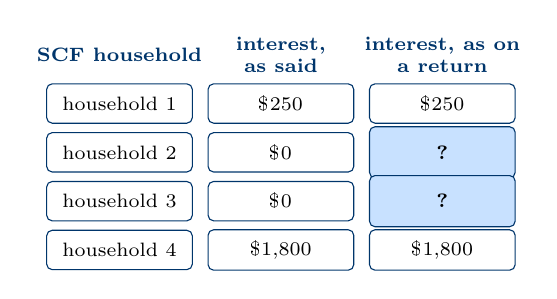
\begin{tikzpicture}[x=2.05cm, y=0.62cm,
          c/.style={tok, minimum width=1.85cm, minimum height=0.5cm, font=\scriptsize}]
        \node[font=\scriptsize\bfseries, text=yaleblue] at (1,0) {SCF household};
        \node[font=\scriptsize\bfseries, text=yaleblue, align=center] at (2,0) {interest,\\as said};
        \node[font=\scriptsize\bfseries, text=yaleblue, align=center] at (3,0) {interest, as on\\a return};
        \foreach \r/\said/\ret/\hd in {1/\$250/\$250/0, 2/\$0/?/1, 3/\$0/?/1, 4/{\$1,800}/{\$1,800}/0} {
          \node[c] at (1,-\r) {household \r};
          \node[c] at (2,-\r) {\said};
          \ifnum\hd=1 \node[c, blank, font=\scriptsize\bfseries] at (3,-\r) {\ret}; \else \node[c] at (3,-\r) {\ret}; \fi
        }
      \end{tikzpicture}

      \vspace{0.8em}
      \small
      The answer given is kept. A second slot holds what the return would show,
      the only slot the PUF has.
    \end{column}
    \begin{column}{0.46\textwidth}
      \centering
      \small
      \begin{tabular}{lrrr}
        \toprule
        Per 100 couples & PUF & SCF & Fill in \\
        \midrule
        \$1--100      & 28 & 8 & 20 \\
        \$100--500    & 13 & 6 & 7 \\
        \$500--2k     & 4  & 3 & 2 \\
        \$2k and over & 3  & 3 & 0 \\
        \midrule
        Any           & 48 & 21 & 28 \\
        \bottomrule
      \end{tabular}

      \vspace{0.8em}
      The PUF sets how many are filled in, and at what sizes.
      The rest of the SCF record sets which households.
    \end{column}
  \end{columns}
  \slidenote{Married, wages \$75--200k. 2015 PUF and 2016 SCF (tax year 2015), weighted. Rows may not add because of rounding.}
\end{frame}

\begin{frame}{Other challenges}
  \begin{itemize}
    \item \textbf{Building tax units from surveys.} Surveys count households. Each one is split
          into tax units by the same rules for every survey, and then we decide who files.
    \vspace{0.5em}
    \item \textbf{The return itself changes.} TCJA cut back itemizing; new items, like the
          tips and overtime deductions, are on no past return.
    \vspace{0.5em}
    \item \textbf{A thin top.} Few very rich records in any source.
    \vspace{0.5em}
    \item \textbf{Future years.} No microdata, only a handful of projected totals.
    \vspace{0.5em}
    \item \textbf{Checking the result.} No source has every variable, so some relationships
          have nothing to check against.
  \end{itemize}
\end{frame}

% ===========================================================================
% 6. Where we are
% ===========================================================================

\begin{frame}{Where we are}
  \begin{itemize}
    \item A 2019 file: 400,000 filer records, plus non-filers
    \vspace{0.4em}
    \item Five sources: the 2015 PUF, the SCF, the CEX, the CPS and the SIPP, every survey
          split into tax units by the same rules
    \vspace{0.4em}
    \item Every PUF item, plus a balance sheet, consumption, tips and auto loan interest
    \vspace{0.4em}
    \item About 750 targets, all met within their standard errors: IRS tables by AGI,
          filing status and age, the top 1\%, 0.1\% and 0.01\%, W-2 tips, SCF wealth
  \end{itemize}
\end{frame}

\begin{frame}{What is left}
  \begin{itemize}
    \item Rules applied after drawing: credit eligibility, death probabilities, unrealized gains,
          the basis of capital gains
    \vspace{0.4em}
    \item The file Tax-Simulator reads, and a first run of Tax-Simulator on it
    \vspace{0.4em}
    \item A tax calculator inside post-training, for targets on computed tax
    \vspace{0.4em}
    \item Other years: 2015 to 2023, then the projection years
    \vspace{0.4em}
    \item The very top: the PUF's aggregate records and the Forbes 400
  \end{itemize}
\end{frame}

\begin{frame}[plain,noframenumbering,c]
  \begin{center}
    {\color{yaleblue}\Large\bfseries Questions}
  \end{center}
\end{frame}

% ---------------------------------------------------------------------------
% Parked: the 24 October intro slides, kept in case any are wanted back.
% ---------------------------------------------------------------------------
\iffalse

\begin{frame}{What do we need?}
  % Click 1: the need as one sentence. Click 2: its words down the side, each explained.
  \only<1>{%
    \vfill
    \begin{center}
      {\LARGE\bfseries\color{yaleblue} Realistic synthetic augmented tax unit microdata}
    \end{center}
    \vfill
  }
  \only<2>{%
  \vspace{0.6em}
  \renewcommand{\arraystretch}{1.4}
  \begin{tabular}{@{}r@{\hspace{1.2em}}>{\raggedright\arraybackslash}p{0.74\textwidth}@{}}
    {\large\bfseries\color{yaleblue} Realistic}   & joint distributions across all variables are respected; aggregate targets are hit \\
    {\large\bfseries\color{yaleblue} Synthetic}   & files for historical and future years \\
    {\large\bfseries\color{yaleblue} Augmented}   & variables not on tax returns, and people who don't file \\
    {\large\bfseries\color{yaleblue} Tax unit}    & the unit that files or would file: non-filers included, households split \\
    {\large\bfseries\color{yaleblue} Microdata}   & individual records, so we can calculate taxes in detail \\
  \end{tabular}
  }
\end{frame}

% What each source has, and which years. Simplified: shading marks whether a
% source carries the item at all, not how well. Tax years.
\begin{frame}{What do we have?}
  \centering
  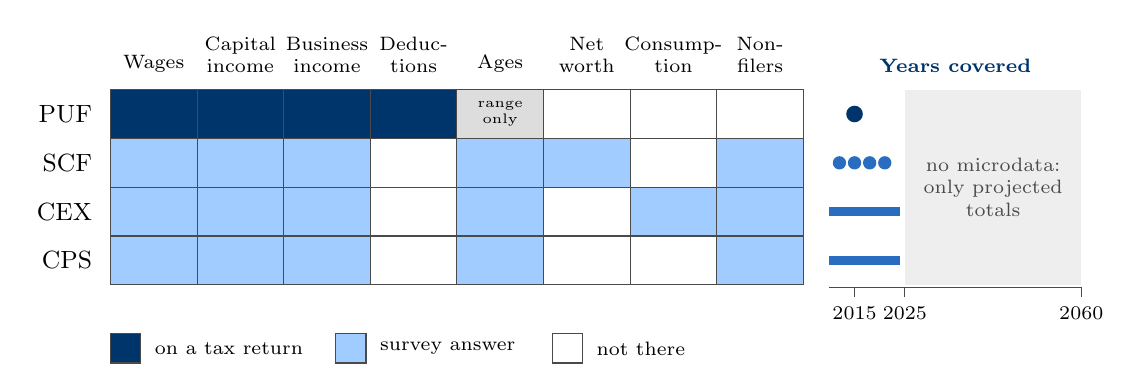
\begin{tikzpicture}[x=1.1cm, y=0.62cm]
    % column labels
    \foreach \lab [count=\i] in {Wages, {Capital\\income}, {Business\\income}, {Deduc-\\tions},
        Ages, {Net\\worth}, {Consump-\\tion}, {Non-\\filers}} {
      \node[font=\scriptsize, align=center, anchor=south] at (\i-0.5, 0.15) {\lab};
    }
    % rows: F = on a tax return, P = survey answer, N = not there
    \foreach \lab/\codes [count=\j] in {
        PUF/{cF,cF,cF,cF,cN,cN,cN,cN},
        SCF/{cP,cP,cP,cN,cP,cP,cN,cP},
        CEX/{cP,cP,cP,cN,cP,cN,cP,cP},
        CPS/{cP,cP,cP,cN,cP,cN,cN,cP}} {
      \node[font=\small, anchor=east] at (-0.1, -\j+0.5) {\lab};
      \foreach \c [count=\i] in \codes {
        \draw[\c, draw=yalegrey] (\i-1, -\j) rectangle (\i, -\j+1);
      }
    }
    % the PUF has the primary filer's age range only, and for most records
    \fill[yalelightgrey] (4,-1) rectangle (5,0);
    \draw[yalegrey] (4,-1) rectangle (5,0);
    \node[font=\tiny, align=center] at (4.5,-0.5) {range\\only};
    % legend
    \begin{scope}[shift={(0,-5.6)}]
      \draw[cF, draw=yalegrey] (0,0) rectangle (0.35,0.6);
      \node[font=\scriptsize, anchor=west] at (0.4,0.3) {on a tax return};
      \draw[cP, draw=yalegrey] (2.6,0) rectangle (2.95,0.6);
      \node[font=\scriptsize, anchor=west] at (3.0,0.3) {survey answer};
      \draw[cN, draw=yalegrey] (5.1,0) rectangle (5.45,0.6);
      \node[font=\scriptsize, anchor=west] at (5.5,0.3) {not there};
    \end{scope}

    % Click 2: which years each source covers, on a line from 2010 to 2060
    \onslide<2>{
    \begin{scope}[shift={(8.3,0)}, x=0.064cm]
      \node[font=\scriptsize\bfseries, text=yaleblue, anchor=south] at (25,0.15) {Years covered};
      % no microdata after the last survey year
      \fill[yalelightgrey!50] (15,-4.0) rectangle (50,0);
      \node[font=\scriptsize, align=center, text=yalegrey] at (32.5,-2) {no microdata:\\only projected\\totals};
      % PUF: 2015 only
      \fill[yaleblue] (5,-0.5) circle (3pt);
      % SCF: every third tax year
      \foreach \yr in {2012,2015,2018,2021} \fill[yalemid] (\yr-2010,-1.5) circle (2.4pt);
      % CEX and CPS: every year
      \draw[yalemid, line width=3pt] (0,-2.5) -- (14,-2.5);
      \draw[yalemid, line width=3pt] (0,-3.5) -- (14,-3.5);
      % axis under the last row
      \draw[yalegrey] (0,-4.05) -- (50,-4.05);
      \foreach \yr in {2015, 2025, 2060} {
        \draw[yalegrey] (\yr-2010,-4.05) -- (\yr-2010,-4.25);
        \node[font=\scriptsize, anchor=north] at (\yr-2010,-4.25) {\yr};
      }
    \end{scope}
    }
  \end{tikzpicture}

  \vspace{0.6em}
  No source has everything, and only one year has tax returns.
  \slidenote{Simplified. Years are tax years.}
\end{frame}

\begin{frame}{Why can't we just combine them?}
  \begin{itemize}
    \item \textbf{Different units.} Surveys count households; returns count tax units.
          One household can hold several returns, and some people file none.
    \vspace{0.6em}
    \item \textbf{Different definitions.} A return caps capital losses at \$3,000;
          survey wages are counted before pre-tax deductions.
    \vspace{0.6em}
    \item \textbf{Different measurement.} Small amounts go unreported: of every 100 couples,
          48 show interest on their returns, but only 21 tell the SCF they have any.
  \end{itemize}
  \slidenote{Interest: married couples with wages of \$75--200k, 2015 PUF and 2016 SCF (tax year 2015), weighted.}
\end{frame}

\begin{frame}{The task}
  \centering
  \vspace{1.5em}
  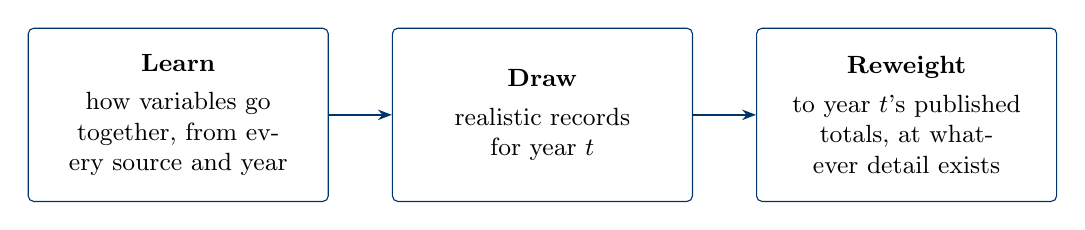
\begin{tikzpicture}
    \node[box, text width=3.6cm, minimum height=2.2cm, font=\small] (learn)
      {\textbf{Learn}\\[3pt] how variables go together, from every source and year};
    \node[box, text width=3.6cm, minimum height=2.2cm, font=\small, right=0.8cm of learn] (draw)
      {\textbf{Draw}\\[3pt] realistic records for year $t$};
    \node[box, text width=3.6cm, minimum height=2.2cm, font=\small, right=0.8cm of draw] (hit)
      {\textbf{Reweight}\\[3pt] to year $t$'s published totals, at whatever detail exists};
    \draw[arr] (learn) -- (draw);
    \draw[arr] (draw) -- (hit);
  \end{tikzpicture}
\end{frame}

\fi

\end{document}
